\documentclass{article}
\iffalse
This file is protected by Copyright. Please refer to the COPYRIGHT file
distributed with this source distribution.

This file is part of OpenCPI <http://www.opencpi.org>

OpenCPI is free software: you can redistribute it and/or modify it under the
terms of the GNU Lesser General Public License as published by the Free Software
Foundation, either version 3 of the License, or (at your option) any later
version.

OpenCPI is distributed in the hope that it will be useful, but WITHOUT ANY
WARRANTY; without even the implied warranty of MERCHANTABILITY or FITNESS FOR A
PARTICULAR PURPOSE. See the GNU Lesser General Public License for more details.

You should have received a copy of the GNU Lesser General Public License along
with this program. If not, see <http://www.gnu.org/licenses/>.
\fi

\author{} % Force author to be blank
%----------------------------------------------------------------------------------------
% Paper size, orientation and margins
%----------------------------------------------------------------------------------------
\usepackage{geometry}
\geometry{
	letterpaper,			% paper type
	portrait,				% text direction
	left=.75in,				% left margin
	top=.75in,				% top margin
	right=.75in,			% right margin
	bottom=.75in			% bottom margin
 }
%----------------------------------------------------------------------------------------
% Header/Footer
%----------------------------------------------------------------------------------------
\usepackage{fancyhdr} \pagestyle{fancy} % required for fancy headers
\renewcommand{\headrulewidth}{0.5pt}
\renewcommand{\footrulewidth}{0.5pt}
\rhead{\small{ANGRYVIPER Team}}
%----------------------------------------------------------------------------------------
% Appendix packages
%----------------------------------------------------------------------------------------
\usepackage[toc,page]{appendix}
%----------------------------------------------------------------------------------------
% Defined Commands & Renamed Commands
%----------------------------------------------------------------------------------------
\renewcommand{\contentsname}{Table of Contents}
\renewcommand{\listfigurename}{List of Figures}
\renewcommand{\listtablename}{List of Tables}
\newcommand{\todo}[1]{\textcolor{red}{TODO: #1}\PackageWarning{TODO:}{#1}} % To do notes
\newcommand{\code}[1]{\texttt{#1}} % For inline code snippet or command line
%----------------------------------------------------------------------------------------
% Various pacakges
%----------------------------------------------------------------------------------------
\usepackage{hyperref} % for linking urls and lists
\usepackage{graphicx} % for including pictures by file
\usepackage{listings} % for coding language styles
\usepackage{rotating} % for sideways table
\usepackage{pifont}   % for sideways table
\usepackage{pdflscape} % for landscape view
%----------------------------------------------------------------------------------------
% Table packages
%----------------------------------------------------------------------------------------
\usepackage{tabularx} % c=center,l=left,r=right,X=fill
\usepackage{float}
\floatstyle{plaintop}
\usepackage[tableposition=top]{caption}
\newcolumntype{P}[1]{>{\centering\arraybackslash}p{#1}}
\newcolumntype{M}[1]{>{\centering\arraybackslash}m{#1}}
%----------------------------------------------------------------------------------------
% Block Diagram / FSM Drawings
%----------------------------------------------------------------------------------------
\usepackage{tikz}
\usetikzlibrary{shapes,arrows,fit,positioning}
\usetikzlibrary{automata} % used for the fsm
%----------------------------------------------------------------------------------------
% Colors Used
%----------------------------------------------------------------------------------------
\usepackage{colortbl}
\definecolor{blue}{rgb}{.7,.8,.9}
\definecolor{ceruleanblue}{rgb}{0.16, 0.32, 0.75}
\definecolor{drkgreen}{rgb}{0,0.6,0}
\definecolor{deepmagenta}{rgb}{0.8, 0.0, 0.8}
\definecolor{cyan}{rgb}{0.0,0.6,0.6}
\definecolor{maroon}{rgb}{0.5,0,0}
%----------------------------------------------------------------------------------------
% Update the docTitle and docVersion per document
%----------------------------------------------------------------------------------------
\def\docTitle{Component Data Sheet}
\def\docVersion{1.3}
%----------------------------------------------------------------------------------------
\date{Version \docVersion} % Force date to be blank and override date with version
\title{\docTitle}
\lhead{\small{\docTitle}}

\def\comp{ad5662}
\def\Comp{AD5662}
\graphicspath{ {figures/} }

\begin{document}

\section*{Summary - \Comp}
\begin{tabular}{|c|M{13.5cm}|}
	\hline
	\rowcolor{blue}
	                  &                                      \\
	\hline
	Names              & \comp                        \\
	\hline
	Worker Types       & Device \\
	\hline
	Version           & v\docVersion \\
	\hline
	Release Date      & January 2018 \\
	\hline
	Component Library & ties.bsp.e310.devices  \\
	\hline
	Workers           & \comp.hdl                \\
	\hline
	Tested Platforms  & xsim, E310(PL)                       \\
	\hline
\end{tabular}

\section*{Worker Implementation Details}
The \comp\ device worker is used to configure the \comp\ MicroDAC hardware block. The hardware takes in a digital word and converts it to an analog voltage value based on the number written. The protocol used to write the DAC value to hardware is compatible with SPI. The \comp\ worker will write the DAC value over SPI to the hardware on property write.
\section*{Block Diagrams}
\subsection*{Top level}
\begin{figure}[ht]
	\centerline{\includegraphics[scale=0.75]{\comp_top_level_diagram}}
	\caption{Top level block diagram of the \comp\ device worker and hardware}
	\label{fig:tb}
\end{figure}
\flushleft
\section*{Source Dependencies}
\subsection*{\comp.hdl}
\begin{itemize}
	\item \$\{E310\_REPO\}/hdl/cards/\comp.hdl/\comp.vhd
	\item \$\{E310\_REPO\}/hdl/cards/\comp.hdl/signals.vhd
\end{itemize}

\begin{landscape}
\section*{Component Spec Properties}
	\subsection*{\comp.hdl}
    \begin{scriptsize}
    	\begin{tabular}{|p{3.75cm}|p{1.25cm}|p{2cm}|p{2.75cm}|p{1.5cm}|p{1.5cm}|p{1cm}|p{6.23cm}|}
        \hline
        \rowcolor{blue}
        Name & Type & SequenceLength & ArrayDimensions & Accessibility & Valid Range & Default & Usage \\
        \hline
        - & - & - & - & - & - & - & - \\
        \hline
        \end{tabular}
    \end{scriptsize}

\section*{Worker Interfaces}
	\subsection*{\comp.hdl}
	\begin{scriptsize}
		\begin{tabular}{|c|c|c|c|c|c|c|c|p{8.5cm}|}
			\hline
			\rowcolor{blue}
			Scope        & Name                 & Type  & SequenceLength & ArrayDimensions & Accessibility     & Valid Range & Default & Usage \\
			\hline
			Property     & \verb+voltageScale+  & ulong & -              & -               & Writable,Readable & 0-32767     & -       & Word to write down to the \comp\ hardware block. Bits 15..0 represent D in the following equation \(V_{out}=V_{ref} (\frac{D}{65536})\), bits 18..16 represent the shutdown mode, and bits 31..19 are don't-cares.    \\
			\hline
		\end{tabular}
	\end{scriptsize}

\section*{Signals}
	\subsection*{\comp.hdl}
	\begin{scriptsize}
			\begin{tabular}{|c|c|c|c|p{2.6cm}|c|c|c|}
			\hline
			\rowcolor{blue}
			Name & Type  & Width & Description \\
			\hline
			TUNE\_DAC\_SYNC  & Out & 1     & SYNC line for SPI connection to \comp\ hardware    \\
			\hline
			TUNE\_DAC\_SCLK  & Out & 1     & SCLK line for SPI connection to \comp\ hardware    \\
			\hline
			TUNE\_DAC\_SDIN  & Out & 1     & SDIN line for SPI connection to \comp\ hardware    \\
			\hline
			VCTCXO\_TO\_MB  & In & 1     & Resultant clock    \\
			\hline
		\end{tabular}
	\end{scriptsize}
\end{landscape}

\section*{Control Timing and Signals}
The \comp\ device worker uses the standard Control Plane signals and the raw property interface.

\section*{Performance and Resource Utilization}
\subsubsection*{\comp.hdl}
\begin{scriptsize}
	\begin{tabular}{|c|c|c|c|c|c|}
		\hline
		\rowcolor{blue}
		Device             & Registers & LUTs & Fmax        & Memory/Special Functions & Design Suite \\
		\hline
		Zynq XC7Z020-1-CLG484 & 38      & 51  & 168.350 & N/A                         & Vivado 2017.1/SDK 2013.4    \\
		\hline
	\end{tabular}
\end{scriptsize}

\section*{Test and Verification}
The testbench for this device worker is meant to analyze the properties of the device worker in a simulation environment. An emulator of the \comp\ hardware was written in order to be able to inspect the timing of the SPI and ensure the transaction was written properly. ocpirun is used to launch the application and then ocpiview is used to analyze the results via manual inspection. The timing diagram should show the property value clocked in on the falling edge of the clock. The data word is formatted as 23..18 don't-cares, 17..16 power down mode bits, and 15..0 data bits.
\\\medskip
The following steps are taken in the testbench:
	\begin{itemize}
		\item[1.] Navigate to the \comp.test directory
		\begin{verbatim}		
		$ cd hdl/cards/ad5662.test
		\end{verbatim}
		\item[2.] Build the assembly used in the test:
		\begin{verbatim}		
		$ ocpidev build --hdl-platform xsim		
		\end{verbatim}
		\item[2.] Run the application as follows:
		\begin{verbatim}		
		$ OCPI_LIBRARY_PATH=`.' ocpirun -v -l8 -t3 ad5662-test.xml
		\end{verbatim}
		\item[3.] Run `ocpiview' to start Vivado to analyze the simulation
		\begin{verbatim}		
		$ ocpiview	
		\end{verbatim}
		\item[4.] Add \verb!ftop->ad5662.i->worker->signals! to the wave window
		\item[5.] The timing diagram should look like the following, clocking in the word 0x7afe after 6 don't-care bits and two 0s for shutdown mode
		\begin{figure}[ht]
	\centerline{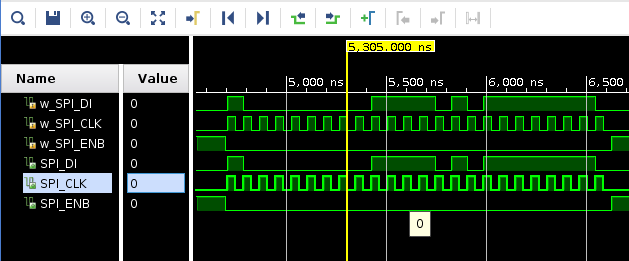
\includegraphics[scale=0.75]{timing}}
	\caption{Timing diagram of a transaction of 0x7afe}
	\label{fig:tb}
\end{figure}
	\end{itemize}

\begin{thebibliography}{2}
\bibitem{usermanual}
  E310 User Manual,
  \url{https://files.ettus.com/manual/page\_usrp\_e3x0.html}.
\bibitem{schematics}
  E310 Hardware Schematics,
  \url{https://files.ettus.com/schematics/e310/}.
\end{thebibliography}

\end{document}
